\documentclass{article}
\usepackage{blindtext}
\usepackage{csvsimple}
\usepackage{graphicx}
\usepackage{hyperref}


\title{NLP Project}
\author{Parsa Kangavari}
\begin{document} 
\maketitle

\section{Phase 1: Crawling And Cleaning Data}
Github Repository Link: \href{https://github.com/rezakongo/soccer_report_analyst}{Click here}.


\subsection{Step 1: Data Crawling}
At first we should find websites that include match reports and player's ratings of a match in a single pages. The best website for this is SkySport.
Then we should find and store urls of that pages. This urls has been crawled from a webpage that contains all matchs. For crawling we use Scrapy framework.
At first we should crawl all URLs from SkySport. So we should crawl urls from a page contains all urls. In this page there will be all urls of all matches.
We should choose seasions that we want. In this project we have chosen Primier league, Champions league and Fifa World Cup.

All matches page link: \href{https://www.skysports.com/premier-league-results}{Click here}.


Then we have been crawled urls of pages contains reports from this page and save them as a csv file. We have developed a spider that do this. you can see it in MatchURLSpider.py.

Results:
\begin{table}
    \begin{center}
        \csvautotabular[]{urls.csv}
    \end{center}
\end{table}


After that we have crawld reports and player ratings from each urls in dataset above. This informations have been crawld by a spider that you can see in SoccerSpider.py.
In this spider we read urls CSV file and then crawl all informations from each url.

Results: 
\begin{table}
    \begin{center}
        \csvautotabular[]{row_data.csv}
    \end{center}
\end{table}

\subsection{Setp 2: Cleaning Data}
For this section we have to clean datas that we crawled before. We should tokenize reports of matchs by sentences and words. 
For first one we split report by dots and for second one we split them by spaces. Then we should clean player ratings. player ratings are in range 0 to 10.
We should set ratings true if they are bigger than 6 and set false otherwise.

tokenized by sentences:

\begin{table}
    \begin{center}
        \csvautotabular[]{sentence_broken_data.csv}
    \end{center}
\end{table}

tokenized by words:

\begin{table}
    \begin{center}
        \csvautotabular[]{word_broken_data.csv}
    \end{center}
\end{table}


\subsection{Step 3: Metrics}
For this section we should get most regular words, unique words of each reports and ... . At first we should create new datasets that contains of 
sentences that belongs to positive and negative players. We have done it in PandNSeperation.py. In this script we seperate sentences belong to negative players 
and positive players and then save them in 2 seperated CSV file; negative and positives.csv.
In this datasets, there are seperated sentences. 

Results for negative:

\begin{table}
    \begin{center}
        \csvautotabular[]{negative_data.csv}
    \end{center}
\end{table}

Results for positives:

\begin{table}
    \begin{center}
        \csvautotabular[]{positive_data.csv}
    \end{center}
\end{table}


Then we should get metrics from that datas. So we write a script thet get all metrics. In SeperatedDataGetMetrics.py all metrics of seperated datas
has been gotten. You can see all metrics as follow:


top10CommonNegativeWordsFrequency:
\begin{center}
    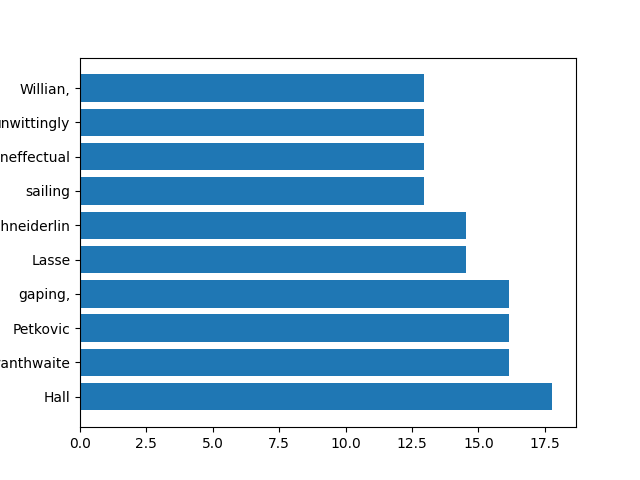
\includegraphics{top10CommonNegativeWordsFrequency}
\end{center}

top10CommonNegativeWordsTFIDF:
\begin{center}
    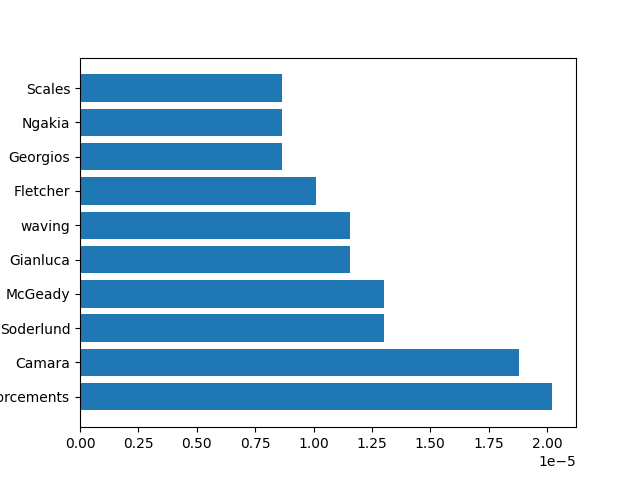
\includegraphics{top10CommonNegativeWordsTFIDF}
\end{center}

top10CommonPositiveWordsFrequency:
\begin{center}
    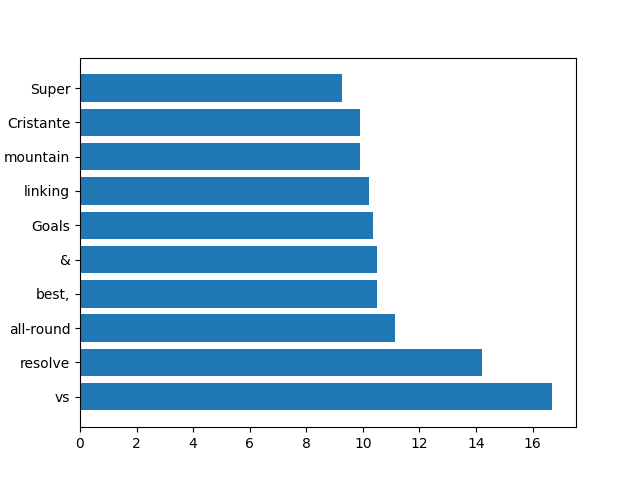
\includegraphics{top10CommonPositiveWordsFrequency}
\end{center}

top10CommonPositiveWordsTFIDF
\begin{center}
    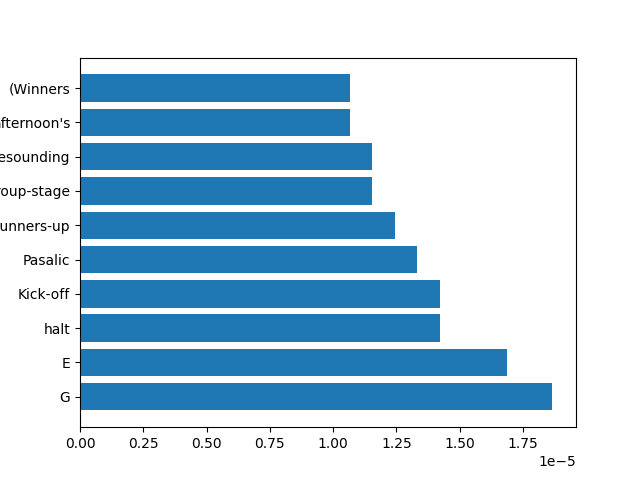
\includegraphics{top10CommonPositiveWordsTFIDF}
\end{center}

top10NegativeWordsCount
\begin{center}
    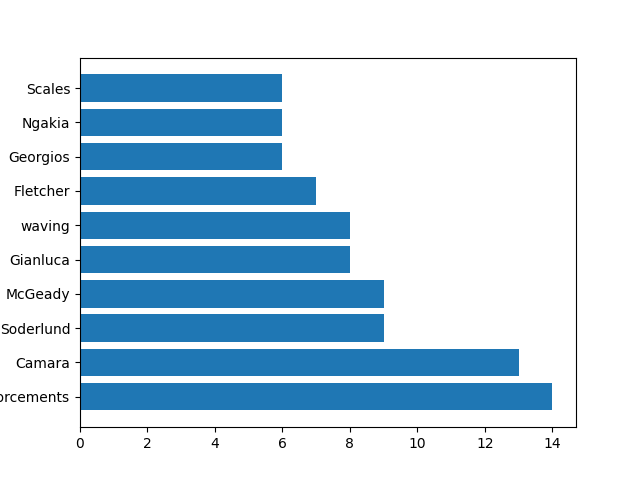
\includegraphics{top10NegativeWordsCount}
\end{center}

top10PositiveWordsCount
\begin{center}
    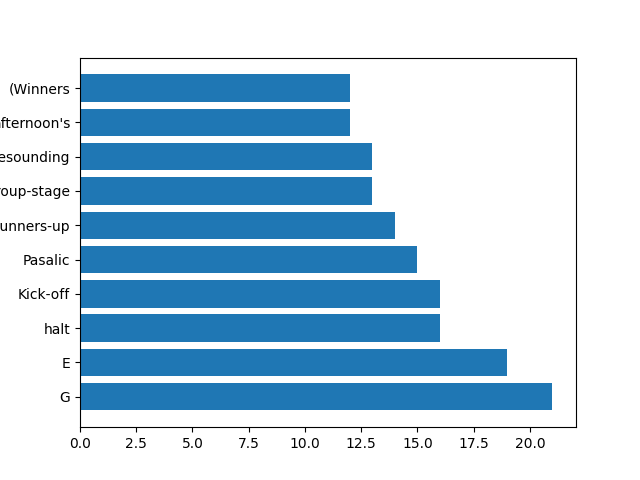
\includegraphics{top10PositiveWordsCount}
\end{center}

After that we should get metrics from new datasets. 
\section{Phase 2: Model Implimentation}
comming soon!
\end{document}